\section{Introduction}

Cette manipulation a pour but la caractérisation d'un module optique (OM) développé pour l'expérience AMANDA. Afin d'étudier les propriétés de cet OM, vous devrez mettre au point le dispositif nécessaire à la prise de mesure. Après avoir pris connaissance avec le dispositif, vous serez ainsi amené à développer vous même la logique d'acquisition des données. Vous analyserez ensuite celles-ci grâce aux outils statistiques et informatiques que vous aurez vu en cours. 

\subsection{Rappel théorique}

\subsubsection{Rayons cosmiques}
La Terre est constamment bombardée par des rayons cosmiques, qui sont des particules chargées dont l'énergie peut atteindre de très hautes énergies ($10^{15}$ à $10^{20}$ eV). Ces rayons cosmiques sont la source de neutrinos atmosphériques. Lorsque les rayons cosmiques pénètre l'atmosphère, les particules primaires produisent des particules secondaires instable avec un temps de vie très court. Ces particules secondaires sont très énergétique et ultra-relativiste. Ces particules secondaires vont soit interagir avec des molécules de l'atmosphère ou se désintégrer en particule plus légère, pour nous donner, entre autre, des muons et des neutrinos.\\

\begin{figure}[h!]
    \center{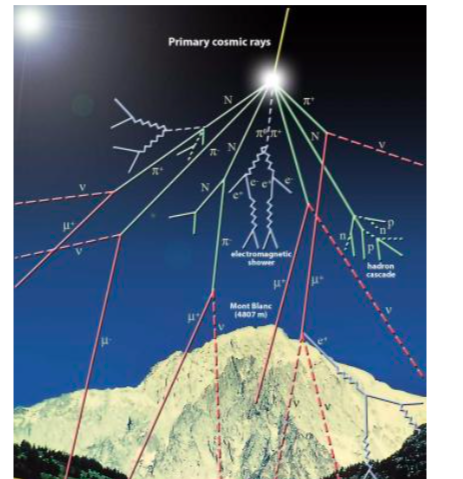
\includegraphics[width=0.56\textwidth]
    {figures/cosmic_rays.png}}
    \caption{\label{fig:CR} Représentation schématique de rayons cosmiques interagissant dans la haute atmosphère.}
\end{figure}

Les muons produits se propagent jusqu'à la surface de la Terre et sont capables de voyager quelques dizaines de kilomètres dans la Terre avant d'interagir. Les neutrinos atmosphériques, quant à eux, peuvent traverser la Terre sans interagir avec un nucléon. Les muons et neutrinos atmosphériques constituent le bruit de fond principal des détecteurs à neutrinos, tel qu'AMANDA et IceCube.

\subsubsection{Effet Tcherenkov}

L'effet Tcherenkov survient lorsqu'une particule chargée se déplace plus vite que la vitesse de la lumière dans un milieu diélectrique. Ce phénomène résulte de la superposition cohérente d'onde électromagnétique suite à la polarisation du milieu par le passage de la particule chargée.

Si la vitesse de la particule est supérieure au ratio $c/n$ (où $n$ est l'indice de réfraction et $c$ la vitesse de la lumière), il y a formation d'un cône de lumière avec un angle de demi-ouverture $\theta_c$ qui suit la relation:

\begin{equation}
    cos\theta_c = \frac{1}{n\beta}
\end{equation}\\

où $\beta = v/c$, $v$ étant la vitesse de la particule dans le milieu. Le nombre de photons Tcherenkov émis par unité de longueur et de longeur d'onde est donné par la formule de Frank-Tamm: \\

\begin{equation}
     \frac{d^2N}{dx \, d\lambda} = \frac{2\pi \, \alpha}{\lambda^2} \; (1- \frac{1}{n^2 \, \beta^2} )
\end{equation}\\

avec $\alpha$ étant la constante de structure-fine. Comme le nombre de photons produits est inversement proportionnel à la longueur d'onde, la contribution des petites longueurs d'onde est plus importante.

\subsubsection{Détecteur Tcherenkov}

Compte tenu de leur faible section efficace d'interaction, la détection des neutrinos nécessite un détecteur de grand volume. Cela est réalisé par les détecteurs Tcherenkov en déployant des photo-multiplicateurs (PMs) dans un volume de matériau diélectrique.\\

\begin{figure}[h!]
    \center{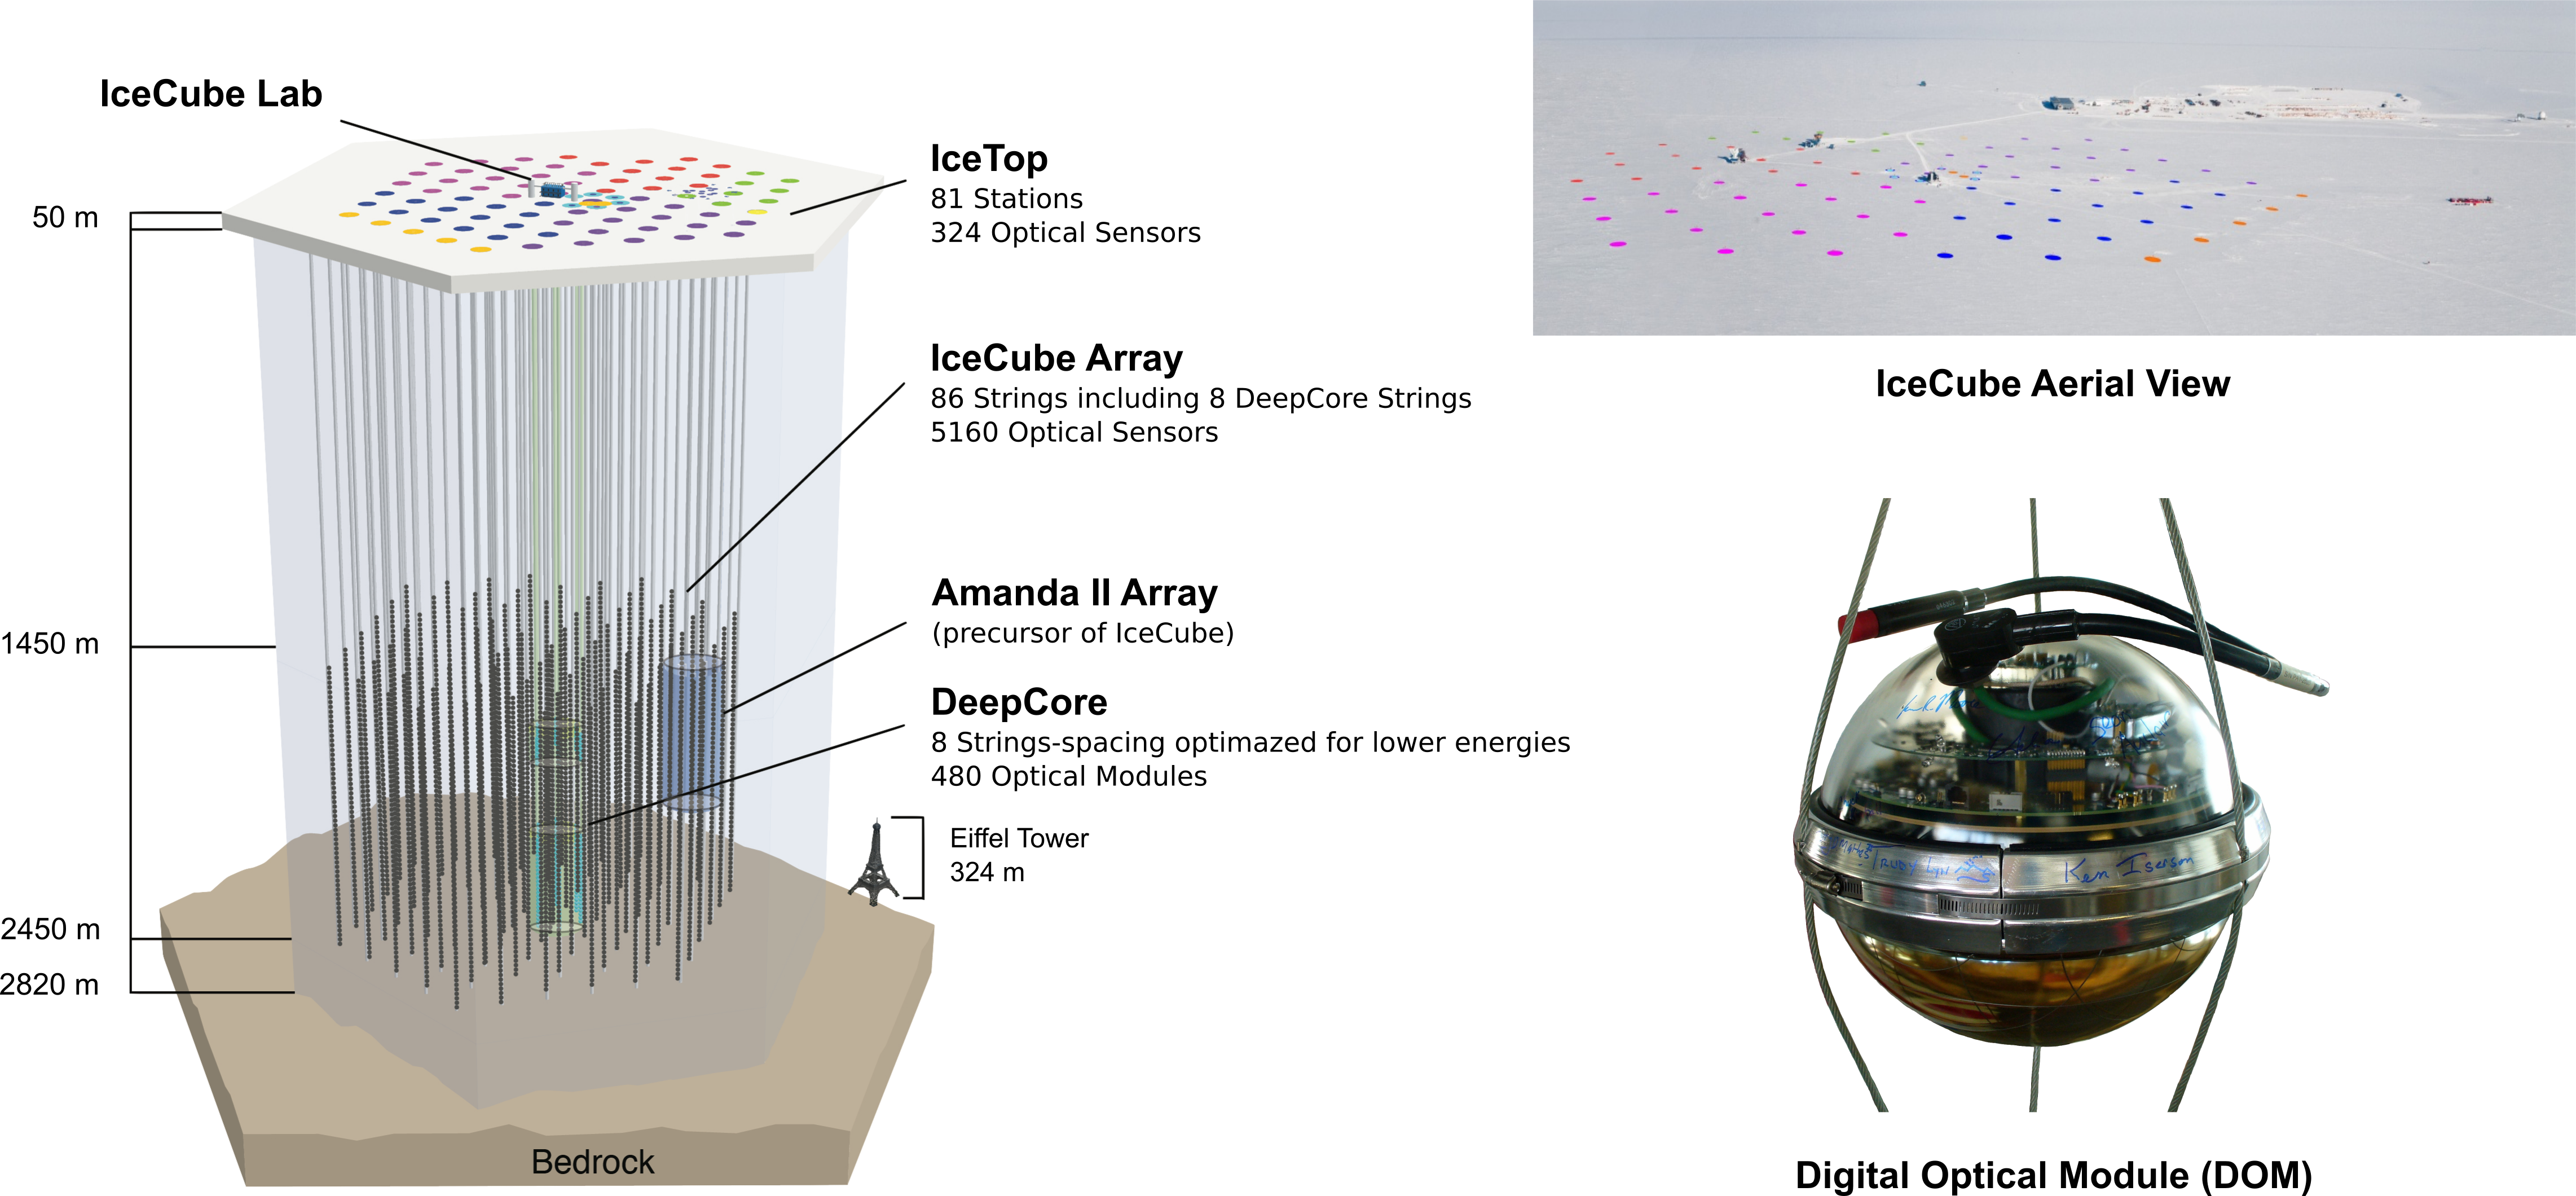
\includegraphics[width=0.9\textwidth]
    {figures/IceCube_Detector.png}}
    \caption{\label{fig:IceCube} Configuration du télescope à neutrinos IceCube.}
\end{figure}

\textbf{AMANDA:}\\
AMANDA (Antarctic Muon and Neutrino Detector Array) est un télescope à neutrino localisé au Pôle Sud. Lors de sa phase finale, le détecteur était composé de 677 modules optiques (OMs) disposés sur 19 câbles. Après 9 ans d'activité, AMANDA a été officiellement incorporé dans au détecteur IceCube en 2005.\\

\textbf{IceCube:}\\
IceCube est un détecteur Tcherenkov d'un kilomètre cube enterré dans la glace du Pôle Sud. Il a pour but principal la détection des neutrinos à haute énergie. IceCube est composé de 5160 modules optiques digitaux (DOMs ou Digital Optical Modules) placés sur 86 câbles.\\

Pour constituer un vaste réseaux d'OMs, il nous faut connaître la réponse de chacun de ceux-ci. Nous allons caractérisé un des modules optiques d'AMANDA à l'aide de dispositifs lors de la conception du détecteur. Contrairement aux modules digitaux (DOMs) d'IceCube, ces OMs nous donneront un signal analogique. 


\subsubsection{Signal type}

Nous allons à présent étudier les différentes composantes d'un spectre en charge typique de la réponse d'un photo-multiplicateur.\\

\begin{figure}[!h]
    \center{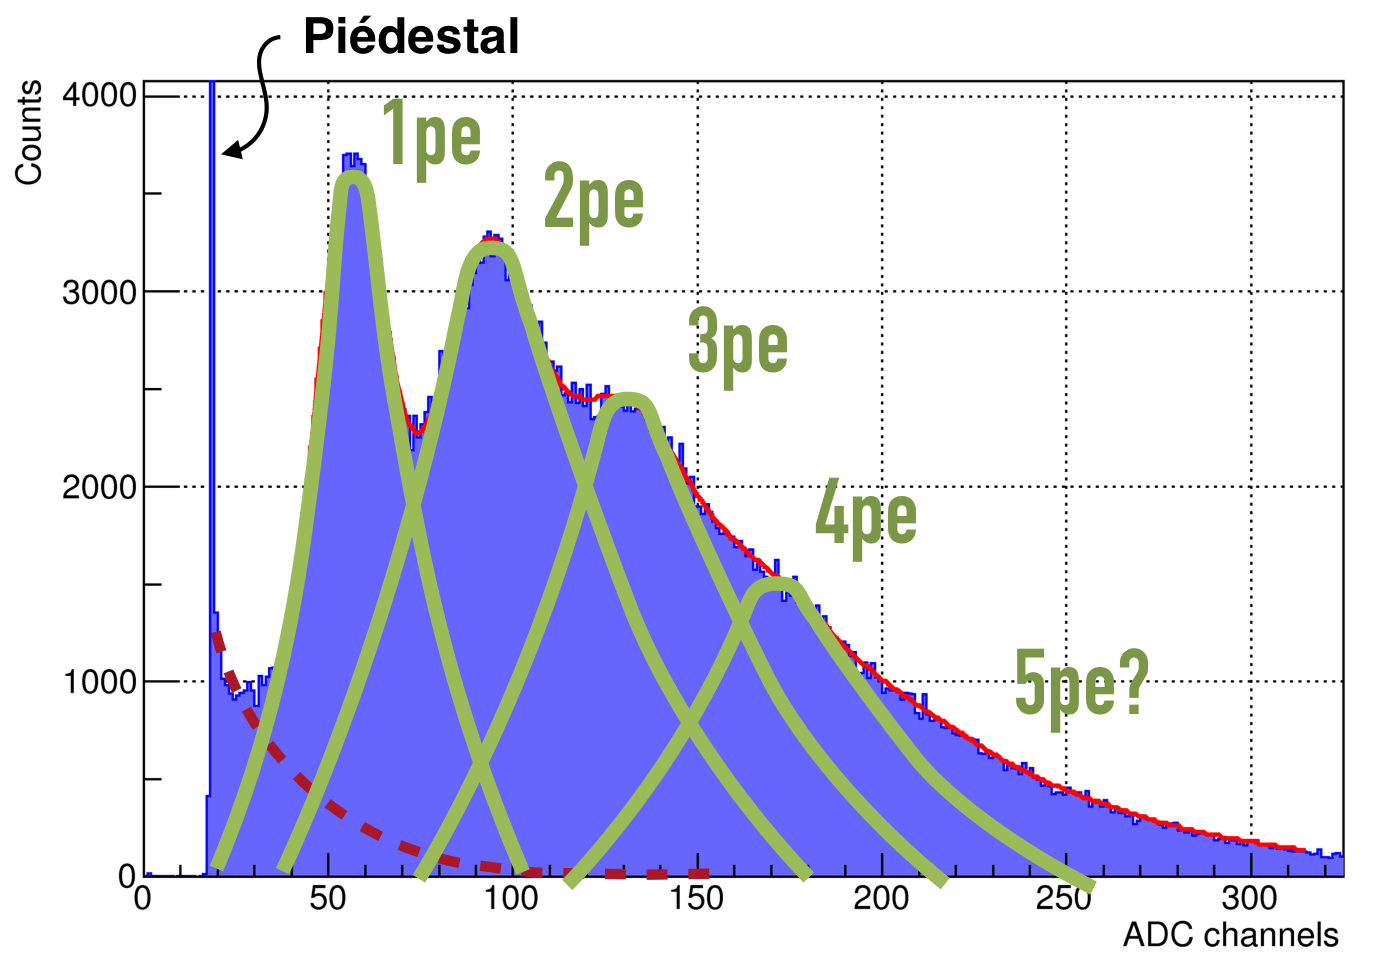
\includegraphics[width=0.7\textwidth]
    {figures/SpectreEnCharge.png}}
    \caption{\label{fig:spectre} Spectre en charge d'un photo-multiplicateur.}
\end{figure}

\textbf{Piédestal :} Il s'agit d'évènements sans charge qui prennent la forme d'un pic en zéro. Afin de se débarrasser de cet effet, il vous faudra régler au mieux votre seuil.\\

\textbf{Dark current :} Il s'agit de bruit associé au PM, il survient lorsqu'un électron est arraché à une dynode sans qu'un photon incident n'arrive à la photo-cathode. Il nous donne une exponentielle décroissante. Cet effet est exacerbé lorsque la tension aux bornes du photo-multiplicateur est élevée. \\

\textbf{Pic des photo-électrons :} Ce sont le réponse en charge du PM pour différent nombre de photo-électrons.\\

Le largeur de la gaussienne du premier photo-électron (1pe) va nous donner la résolution en charge du PM. La relation entre la hauteur des gaussiennes nous est donné par la distribution de Poisson.



\subsection{Agenda du laboratoire}
\textbf{Lundi}
\begin{itemize}
\item Prendre connaissance avec le matériel
\item Vérifier le signal analogique des PMs et la sortie correspondante du discriminateur avec l'oscilloscope.
\item Implémenter de la table de vérité pour la logique d'acquisition ou trigger.
\item En utilisant les scaler NIM, calculer l’éfficacité de PM2 vs PM1 et PM3 (dispositif 2), ou PM1 vs PM2 et OM (dispositif 1) en fonction de la haute tension et du seuil du discriminateur. Mesurer aussi les taux de PM1 (PM2) en fonction de la haute sension et le seuil.
\end{itemize}
\vspace{\baselineskip}
\textbf{Mardi}
\begin{itemize}
\item Calibrer l'ADC: Introduire une charge connue à l'entrée de l’ADC. Prendre des données pour différentes charges avec le logiciel associé. Déterminer le paramètre de conversion de numéro de coups d’ADC vers charge
\item Préparer l'acquisition de données, vérifier avec l'oscilloscope que les signaux et le gate arrivent en même temps à l'ADC.
\item Démarrer l'acquisition de données avec LabView pour obternir le spectre en charge du PMT quand il y a un signal.
\end{itemize}
\vspace{\baselineskip}
\textbf{Mercredi}
\begin{itemize}
\item Construire la logique d'acquisition pour le bruit de fond.
\item Écrire la table de vérité pour définir un événement du bruit.
\item Vérifier que le gate et le signal du PMT arrivent simultanément à l'ADC.
\item Démarrer l'acquisition de données pour obtenir le spectre en charge quand il n'y a pas de signal.
\end{itemize}
\vspace{\baselineskip}
\textbf{Jeudi et Vendredi}
\begin{itemize}
\item Développement d'un programme de génération Monte Carlo d'une distribution normale et faire le fit de votre distribution Monte Carlo.
\item Développement des programmes d'analyse.
\item Dernier jour pour présenter les résultats des exercices.
\item Préparation de la présentation.
\end{itemize}

\pagebreak